%%%%%%%%% PROJECT DESCRIPTION  -- 15 pages (including Prior NSF Support)
\setcounter{page}{1}
\renewcommand{\thepage}{\arabic{page}}
%\section{Project Description}

\invisiblesection{Project Description}
%The Project Description (including Results from Prior NSF Support, which is
%limited to five pages) may not exceed 15 pages. Visual materials, including charts,
%graphs, maps, photographs and other pictorial presentations are included in the
%15-page limitation. PIs be cautioned that the project description must
%be self-contained and that URLs that provide information related to the proposal
%should not be used. \\
%
%All proposals to NSF are reviewed utilizing the two merit review criteria,
%intellectual merit and broader impacts. \\
%
% The Project Description should provide a clear statement of the work 
% to be undertaken and must include: objectives for the period of the proposed 
% work and expected significance; relation to longer-term goals of the PI's 
% project; and relation to the present state of knowledge in the field, 
% to work in progress by the PI under other support and to work in progress 
% elsewhere.

\subsection{Motivation and Background\label{sec: motivation}}
\changliu{Tentative title: Domain-specific benchmarks for \tomi{intelligent} industrial collaborative robots}

\liting{make this a figure - high-level intelligence
monitor, cooperation, imitation, dexterity $->$ efficiency; 
hierarchical structure
goal: efficiency
interaction awareness: peer-peer (cooperation, remote?), master (monitor: product quality, procedure, co-worker common working patterns), slave (imitation: domain-specific learning)
dexterity (self): 1) finish the task; 2) express self via audio and gestures.
(add example figures to demonstrate)
(example: assembly and surface processing)}

Human-robot collaboration is one of the most promising field for future robotics. Instead of being isolated from human, robots of the future are envisioned to interact closely with human to better serve, assist and collaborate with people in our daily lives across work, home and leisure. Human-robot collaboration is happening in various fields. This proposal is focused on industrial domain. It is observed that the emphasis in manufacturing is shifting from mass production to mass customization, as consumers' interest in personalized products keeps increasing \cite{pine1999mass}. In response to such shifts, many research and development efforts have been directed to flexible automation \cite{hutchinson1982economic,jovane2003present}. However, it is difficult to make the current production lines with robots truly flexible, due to the rigidity of the current generation of industrial robots. On the other hand, including human workers in the human-robot teams will bring flexibility, intelligence and versatility to automation.


\liting{To enable this goal, different levels of intelligence are desired: from high-level intelligence such as automatic task generation to low-level intelligence such as trajectory tracking via feedback.} Recent advances in the robotics have brought huge improvements of collaborative robots (co-robots), both in hardware and software. Various methods have been proposed to ensure that they work safely and efficiently with humans. \changliu{Need some literature review here. Point out several large research projects.} \liting{Typically, a standard co-robot contains multiple interacting modules, including physical hardware module, perception module, planning module, and control module. Each modules may has sub-modules. }

However, we observe the following two problems: 1) lack of domain-specific high-level intelligence; 2) lack of standard tools to guide and evaluate different designs. By high-level intelligence, we refer to various skills that the robot can use to improve overall task efficiency. It is domain-specific in multiple aspects. To improve efficiency in human-robot collaboration, the robot needs to not only be dexterous in its own tasks, but also properly play its role in various kinds of interactions. Dexterity refers to both physical skills (to finish tasks) and communication skills (to express intentions). For example, physical skills for industrial co-robots include the understanding of assembly procedures of various products, and the desired  processing parameters for surfaces with various kinds of materials. Human workers also learn these skills gradually from experience. For communication skill, the robot needs to express itself to its human co-workers to avoid misunderstanding. On the other hand, robots can play various kinds of roles during collaborations. They can be peers to humans, masters to monitor human workers, slaves to assist or learn from human workers. In peer-to-peer interaction, robots need intelligence to boost cooperation. When robots are masters, they need to be equipped with the knowledge to monitor human workers' working progress, hence product quality. When robots are slaves, they need to be able to imitate humans' behaviors. The contents of aforementioned high-level intelligence are all deeply related to the specific domain. \changliu{Insert a figure to illustrate high-level intelligence}

\paragraph*{Domain-specific knowledge is needed for high-level intelligence. }~
\changliu{domain knowledge}
\tomi{Need to address what kind of domain-specific knowledge is needed in a given application domain. This is another point for high-level intelligence, and also one kind of the guidance for benchmark. Give some examples; mass customization; four-hand tasks;What human and robots are good at?} 

To address fundamental problems of co-robots, a certain level of abstraction is needed in order for researchers to develop methodologies that cover a wide range of applications. The abstraction indeed creates a gap between the research problem and the specific real world applications. \changliu{Give an example here.} However, as co-robots are to be deployed in the real world, the gap should be bridged at some point. Bringing domain-specific knowledge for high-level intelligence can help to narrow the gap \changliu{Need reference}. \changliu{Give another example here.}   
We propose to equip the robot with the domain-specific knowledge, and enable fast adaptation and learning of domain-specific knowledge. \liting{do we need to say that the ``domain-specific'' knowledge that we focus on is the industrial scenario? Also, I think that we need to explain why domain-specific knowledge is of particularly importance for high-level intelligence.}

\paragraph*{Standard evaluation tools and benchmarks are needed to guide different designs. }~
A co-robot is a complex system that consists of multiple interacting modules. A standard co-robot contains physical hardware module, perception module, planning module, and control module. Modules may have submodules. For example, in a planning module, there can be task planning submodule, motion planning submodule, etc. Different co-robots may have different architectures as well as different designs of corresponding modules. Those inconsistencies lead to several drawbacks.
\begin{enumerate}
	\item It is difficult to \textbf{compare} different designs of co-robots, hence difficult to understand the sources of advantages or disadvantages of various designs, i.e., whether the advantage comes from the architecture or the method used in a specific module.
	\item It is difficult to \textbf{decompose} the complex system to allow researchers from different background to focus on advancing methodologies in the modules of their own expertise and then integrate state-of-the-art results of other parts into their systems. Significant gap in research schemes has been observed between perception community and control community. The co-robot solutions developed in perception community tend to use too simple control strategy and ignores the hardware limitations. The co-robot solutions developed in control community sometimes fail to take the advantage of solutions provided by perception community.
	\item It is difficult to \textbf{coordinate} different modules from the system perspective. The development of co-robots needs to integrate the results from different fields. However, we still lack a perspective and viable tool for system engineering. For example, if the overall system needs to achieve certain objective, what are the sub-objectives of different modules? How can we prove that once the sub-objectives are achieved, the overall objective of the system can then be achieved?
	\item No \textbf{benchmark} problem has been introduced to provide fair comparison of different designs and guidance for new designs. Currently, different designs are tested in different customized scenarios, which greatly limits the transferability and reproducibility of technologies. The difficulty in developing a fair benchmark is that human robot collaboration is intrinsically highly stochastic and domain-specific.  
	We propose to establish a set of principles to evaluate and benchmark different designs of  co-robots in industrial environments. \liting{Is this point also a drawback caused by the inconsistencies?}
\end{enumerate}

\tomi{More high-level intelligence: advanced collaboration. Instead of being passive, the co-robot should be actively responsible for the collaboration process (e.g., product quality should be guaranteed) as well as its collaborators. Robots should be monitoring the collaboration system,  and include some audio feedback and communication (RO2H). If the error made by human is recoverable, then the robot can try to fix it; If not recoverable, then send message. 
\\	
Other possible ideas: wireless communication: for instance, remote learning from demonstration, or remote collaboration (think about a problem)}


In summary, the goal of this project is of two-fold. The first objective is to equip robot with high-level intelligence from domain-specific knowledge. The second objective is to develop and standardize evaluation methods and benchmarks for industrial co-robots.

\subsection{Intellectual Merit}

To achieve intelligent and efficient human-robot collaboration in industrial environments, we propose to 1) equip robot with high-level intelligence, 2) develop methods to evaluate different designs including module-wise verification, inter-modular verification, and system verification, and 3) develop benchmark systems (hardware involved) to validate human-robot collaborations in industrial settings.


\subsection{Summary of the Proposed Work}



\subsection{Technical Background / State of the Art}
\liting{@yujiao, jessica} please check literature reviews accordingly

\subsubsection{High-level Intelligence}
\liting{tentative definitions for different level of intelligence: high-level intelligence aims for efficiency - understanding the tasks and its collaborators (the human); low-level intelligence aims for safety and accuracy - knowing how to act correctly.}

In our definition, high-level intelligence of robots refers to their abilities in understanding the tasks and their collaborators so that they can automatically make or adjust decisions that are beneficial for the efficiency of the collaboration. For example, \liting{an example consistent with our applications}. State-of-the-art high-level intelligence designs can be mainly categorized into two domains: 1) autonomous task scheduling, 2) human intention recognition and 3) human motion prediction (\liting{not sure whether we need this}). For the first domain, \cite{baraglia2016initiative} shows that people collaborate best with a proactive robot which takes initiative, yielding better team fluency and high subjective ratings. \cite{devin2017decisions} even shows in which conditions the robot can determine when it has to take the decision by itself or leave it to its human partner. Thus, when a robot is taking the lead, it is also important for robot to act explicitly and predictably so that plans synthesized by the robot can be easily understood by humans when doing task planning. Zhang et al. \cite{zhang2017plan} use conditional random fields to learn the labeling scheme of human which is to associate abstract tasks with robot actions. Then, they use the learned model to label a new plan to compute its explicability and predictability. These measures can be used by robots to proactively choose or directly synthesize plans that are more explicable and predictable. 

Regarding human intention recognition,  a lot of system architectures have also been proposed. For example, Schrempf et al. \cite{schrempf2005nove} suggest a framework for human robot interaction using human intention recognition with Dynamic Bayesian Networks (DBN). A planner uses minimum entropy to choose between competing human intentions and executes a hand-coded action from a fixed set. Similarly, in \cite{koppula2016anticipatory}, human is modeled through their low-level kinematics as well as their high-level intent. This allows the model to anticipate a belief about possible future human actions. Moreover, the human’s and robot’s behavior are modeled through an Markov decision process. In  the  work  of \cite{devin2016implemented},  starting  from  the  capability  of  the  robot  to permanently compute the spatial perspective of its partners and to track their activity, the robot adaptively manages the execution of shared  plans  in  a  context  of  humans  and  robots  performing  collaborative  objects  manipulation.  As  a result,  the  robot  is  able  to adapt to human’s decisions and actions and to inform them when needed  without  being  intrusive  by  giving (unnecessary)  information that the human can observe or infer by himself. Huang et al. \cite{huang2016anticipatory} propose a robot system that monitors its user's gaze, predicted his or her task intent based on observed gaze patterns, and performed anticipatory task actions according to its predictions. 


\liting{The main ending point of this part is that we need domain-specific knowledge to design better high-level intelligence in industrial applications.}



\begin{comment}
To improve efficiency of human robot interaction, a powerful planner is at the core of the high-level intelligence. If the system is autonomous, the planner should be able to schedule tasks online autonomously and responds flexibly to any explicit commands or implicit intentions on the side of the human user \cite{schrempf2005nove}. However, in industrial scenarios, the system is more common where we can predefine the courses of the human and robot actions, and often human worker has several alternative plans. In this case, one challenge lies in planning the robot action with uncertain knowledge of human intention. 

A lot of system architectures are proposed to cope with this problem by integrating human intention recognition and the planner. 
Schrempf et al. \cite{schrempf2005nove} suggest a framework for human robot interaction using human intention recognition with Dynamic Bayesian Networks (DBN). A planner uses minimum entropy to choose between competing human intentions and executes a hand-coded action from a fixed set. Similarly, in \cite{koppula2016anticipatory}, human is modeled through their low-level kinematics as well as their high-level intent. This allows the model to anticipate a belief about possible future human actions. Moreover, the human’s and robot’s behavior are modeled through an Markov decision process. In  the  work  of \cite{devin2016implemented},  starting  from  the  capability  of  the  robot  to permanently compute the spatial perspective of its partners and to track their activity, the robot adaptively manages the execution of shared  plans  in  a  context  of  humans  and  robots  performing  collaborative  objects  manipulation.  As  a result,  the  robot  is  able  to adapt to human’s decisions and actions and to inform them when needed  without  being  intrusive  by  giving (unnecessary)  information that the human can observe or infer by himself. Huang et al. \cite{huang2016anticipatory} propose a robot system that monitors its user's gaze, predicted his or her task intent based on observed gaze patterns, and performed anticipatory task actions according to its predictions. 

Robot predicting and responding to human is neccesary, and it would be more productive if robot is proactive. \cite{baraglia2016initiative} shows that people collaborate best with a proactive robot which takes initiative, yielding better team fluency and high subjective ratings. \cite{devin2017decisions} even shows in which conditions the robot can determine when it has to take the decision by itself or leave it to its human partner. Thus, when a robot is taking the lead, it is also important for robot to act explicitly and predictably so that plans synthesized by the robot can be easily understood by humans when doing task planning. Zhang et al. \cite{zhang2017plan} use conditional random fields to learn the labeling scheme of human which is to associate abstract tasks with robot actions. Then, they use the learned model to label a new plan to compute its explicability and predictability. These measures can be used by robots to proactively choose or directly synthesize plans that are more explicable and predictable.
\end{comment}

\subsubsection{Theoretical Evaluations}

Apart from high-level intelligence, this work also aims to come up with a framework to evaluate the performance of different co-robot systems. The following sections cover evaluation on the theoretical aspect for both modular level and inter-modular level. 

\paragraph{Modular-wise verification}~

As mentioned in the motivation section, a co-robot system usually contains the following modules: perception module, planning module , and control module. For each module, we investigate the verification approaches in terms of evaluation metrics and frameworks. \liting{we need to discuss about this}

\noindent{\liting{\textbf{Perception Module}:}}
1. evaluation metrics
2. evaluation frameworks

\noindent{\textbf{Planning Module}:} Among all robotics applications, planning module can usually be decomposed into two sub-modules: task planning sub-module and motion planning sub-module. In terms of evaluation metric, time-efficiency for the task planning performance is the most commonly used measure \cite{foster1999influence,edan1991near,galindo2004improving}. \liting{Is that the only one?} The same metric can be evaluated in two different aspects: 1. planning time required for the solver to generate a solution \cite{galindo2004improving} 2. time required to complete the whole task for the generate plan \cite{edan1991near}. Comparing to task planning, a variety of metrics have been proposed for motion planning evaluation, including: 1. computational efficiency \cite{buckley1989fast} which can be evaluated similarly as measuring in task-planning 2. energy efficiency \cite{mei2004energy} which .... , responsiveness \cite{ratliff2009chomp} which ... , feasibility \cite{cowlagi2012hierarchical}, and safety \cite{frazzoli2002real}. In HRI systems, while efficiency is an important measure, feasibility and safety are usually the biggest concerns and are more complected to be evaluated.  In \cite{cowlagi2012hierarchical} 

Several evaluation frameworks have also been proposed. 1. mass test. 2. Simulation test. 
\liting{we need more reference for each case}

\begin{comment}
Researches also proposed that in order to further increase efficiency, task-planning and motion planning should be done together. In \cite{garrett2015ffrob,mahmoudzadeh2016toward}, by incorporating the constraints from geometry and kinematics, these hybrid methods guarantees successful completion of task plans. The previous evaluation methods are applicable in these hybrid methods as well.  
(reason for deleting: not very related)
\end{comment}

\noindent{\textbf{Control Module}:} The control module contains the tracking controllers that allow the robot to carry out the motion planned by the planning module. In terms of evaluation metrics, stability, tracking errors and response time are three commonly used metrics. For example, \liting{add reference here}. Regarding the evaluation frameworks, theoretical analysis is a standard in control module. 

\begin{comment}
In \cite{kanjanawanishkul2009path, falcone2007predictive}, Model Predictive Control (MPC) is used for tracking purpose. As a result of a properly formulated MPC problem, the controllers are guaranteed to bring the tracking error to zero theoretically. Other commonly seen control methods that require empirical parameter-tuning are proposed \cite{kanayama1990stable, xian2004, niu2013barrier}. Stability of these control rules are proved through the use of a Liapunov function. Aside from theoretical guarantees, the performance of these control modules can also be evaluated by simply recording the tracking error.
\end{comment}


\paragraph{Inter-modular verification}~
While each module in a robotic system can be evaluated separately, it is important to check whether these module can also work together effectively. Previously, researchers do not emphasize much on this aspect, however, since the technology for every module has been improved a lot through out the years, there is a bigger verity of modules we can choose from. Although there hasn't been much work focusing on this aspect in the robotics community, people in the autonomous driving area have been research on this for sometime. ...    
methods: 1. accelerated tests. 2. Simulation tests. 3. Mass online tests.
\liting{details coming soon}

\paragraph{System verification}~
In the field of HRI, researchers tend to work toward building a comprehensive robotic system, therefore, evaluation methods regarding the whole system are also more commonly seen. Different from inter-modular evaluation, we include evaluating the effect of human factor to the HRI system when examining the system as a whole.  In \cite{goodrich2008human}, the authors defined HRI systems as a system with several features: autonomy, information exchange, teamwork, adaptation, learning, training, task-shaping, and finding a unifying theme. With these features identified, the HRI system can be evaluated according each aspect. In \cite{steinfeld2006common}, the authors also highlight several features of HRI systems: navigation, perception, management, manipulation, and biasing effects. A list of detailed measures are also included in the paper. These measures are especially useful during the system design process. The authors also provide metrics the evaluate the HRI system: 1. Quantitative performance which takes account of the percentage of the mission that was accomplished and the time required to complete a task. 2. Subjective ratings which is used to assess the quality of the effort and is compiled from all stakeholders involved, both direct and indirect. 3. Appropriate utilization of mixed-initiative which infer the ability of the human-robot team to appropriately regulate who has control initiative. Similar ideas are also proposed in \cite{burke2004final,murphy2013survey}. Some other works focus more on the measures that evaluate the interaction in between human and robots. In \cite{goodrich2008human}, the authors specify interaction time, mental workload, and situation awareness produced by the interaction between the human and the robot as the measures of efficiency. In \cite{steinfeld2006common}, interaction characteristics, persuasiveness, trust, engagement, and compliance are features for evaluation towards effects introduced by human. There are works especially focusing on HRI system in industrial settings \cite{michalos2018method,takata2011human,chen2011assembly}. In \cite{michalos2018method}, the system is examined from many aspects that are more industry oriented: robot reach, strength criterion, robot payload, ergonomic criteria, cost, investment cost, floor space, time saturation, fatigue, and handling time that are quite different from the focus of academic HRI research.

\subsubsection{Benchmarks on Industrial Settings}

As technology improves, it is getting clearer that human-robot collaborative work space will be one of the common scenes in future factories. Therefore, having a stander benchmark to evaluate HRI systems in industrial settings has become important than ever before. A work shop in IROS 2015 aimed to advance the topic of benchmarking in HRI system in the area of industrial settings \cite{dalgaard2015workshop}. It is mentioned that while HRI evaluation are scattered in a myriad of different approaches and ways of performing and testing, the community is still missing consensus tools to standardized assessment of robot products and applications in use in terms of safety, performance, user experience, and ergonomics. Comparing to benchmark system in industrial settings, benchmarks for domestic service robots
have been around for a longer time \cite{wisspeintner2009robocup}. A more recent paper discussed the result of a survey about researchers' opinion toward common metrics and benchmarks in HRI \cite{aly2017metrics}. In this paper, the Turing test \cite{turing2009computing}, Winograd schemas \cite{levesque2011winograd}, RoboCup Soccer \cite{kitano1998robocup}, and RoboCup@Home \cite{wisspeintner2009robocup} are listed as the performance benchmarks. Although some of the ideas might be similar to those for industrial settings, it is also true that we need new benchmarks for industrial scenarios. Since the robots in the industrial settings are usually larger in scale and more powerful in generating force, safety naturally becomes the biggest concern in the evaluation. One of the few works cover benchmarking suitable for industrial settings \cite{de2008atlas}, if not the only one, also focuses on safety aspect. Based on the existing benchmark frameworks for other HRI scenarios, the author mentioned including the manipulator safety index (MSI) \cite{zinn2004playing} which is based on head injury criterion (HIC) \cite{versace1971review} and is widely used in industry. In \cite{rosen2018evaluation}, the authors also incorporate many existed criteria in the industrial HRI design. These results suggest that we should consider the commonly used criteria in industry to design the benchmark setting and collect benchmark data, which do not exist in the industrial HRI community yet.   

\subsection{Prior Work by the Principal Investigator}



\subsubsection{RSIS}
The PIs have introduced the robot safe interaction system (RSIS) \cite{liu2018robot}, which establishes a methodology to design the robot behavior to \textbf{safely and efficiently} interact with humans. In order to address the uncertainties during human-robot interactions, a unique parallel planning and control architecture is introduced, which has a long term global planner to ensure efficiency of robot behavior, and a short term local planner to ensure real time safety under uncertainties. The parallel planner integrates fast algorithms for real-time motion planning, e.g. the convex feasible set algorithm (CFS) \cite{liu2017sicon} for the long term planning, and the safe set algorithm (SSA) \cite{liu2014control} for the short term planning. 
\changliu{Will add two figures here: 1. architecture. 2. result}


\subsubsection{SERoCS}
Based on RSIS, the PIs further introduced safe and efficient robot collaboration system (SERoCS) which include more high-level intelligence to the robot.
\subsubsection{Benchmarks}

\subsection{Proposed Work}







\subsection{Project Schedule}





\subsection{Broader Impacts, Proposed Educational Plan, and Outreach}
% As in the project summary, broader impacts must be called out separately 
% in the project description.  You may be able to give more specific
% examples, or discuss how you've previously achieved these impacts.
% It should be similar, but not identical, to the Broader Impacts statement
% in the project summary

%\begin{wrapfigure}{r}{5cm}
%\vspace{-18pt}
%  \begin{center}
%  \subfloat[The evaluation environment on Platform 1, Task a.2.2. The robot needs to pick the workpiece (marked as star) in the tray. The human is moving around.\label{fig: preliminary}]{
%    \includegraphics[width=5cm]{src/environment}}\\
%   \subfloat[Illustration of the resulting robot trajectory using the proposed robot brain.\label{fig: trajectory}]{\includegraphics[width=5cm]{src/trajectory}}
%  \end{center}
%  \vspace{-20pt}
%  \caption{Preliminary study.}
%  \vspace{-10pt}
%\end{wrapfigure}


\paragraph*{General}~

\begin{wrapfigure}{R}{4.5cm}
\vspace{-25pt}
  \begin{center}
    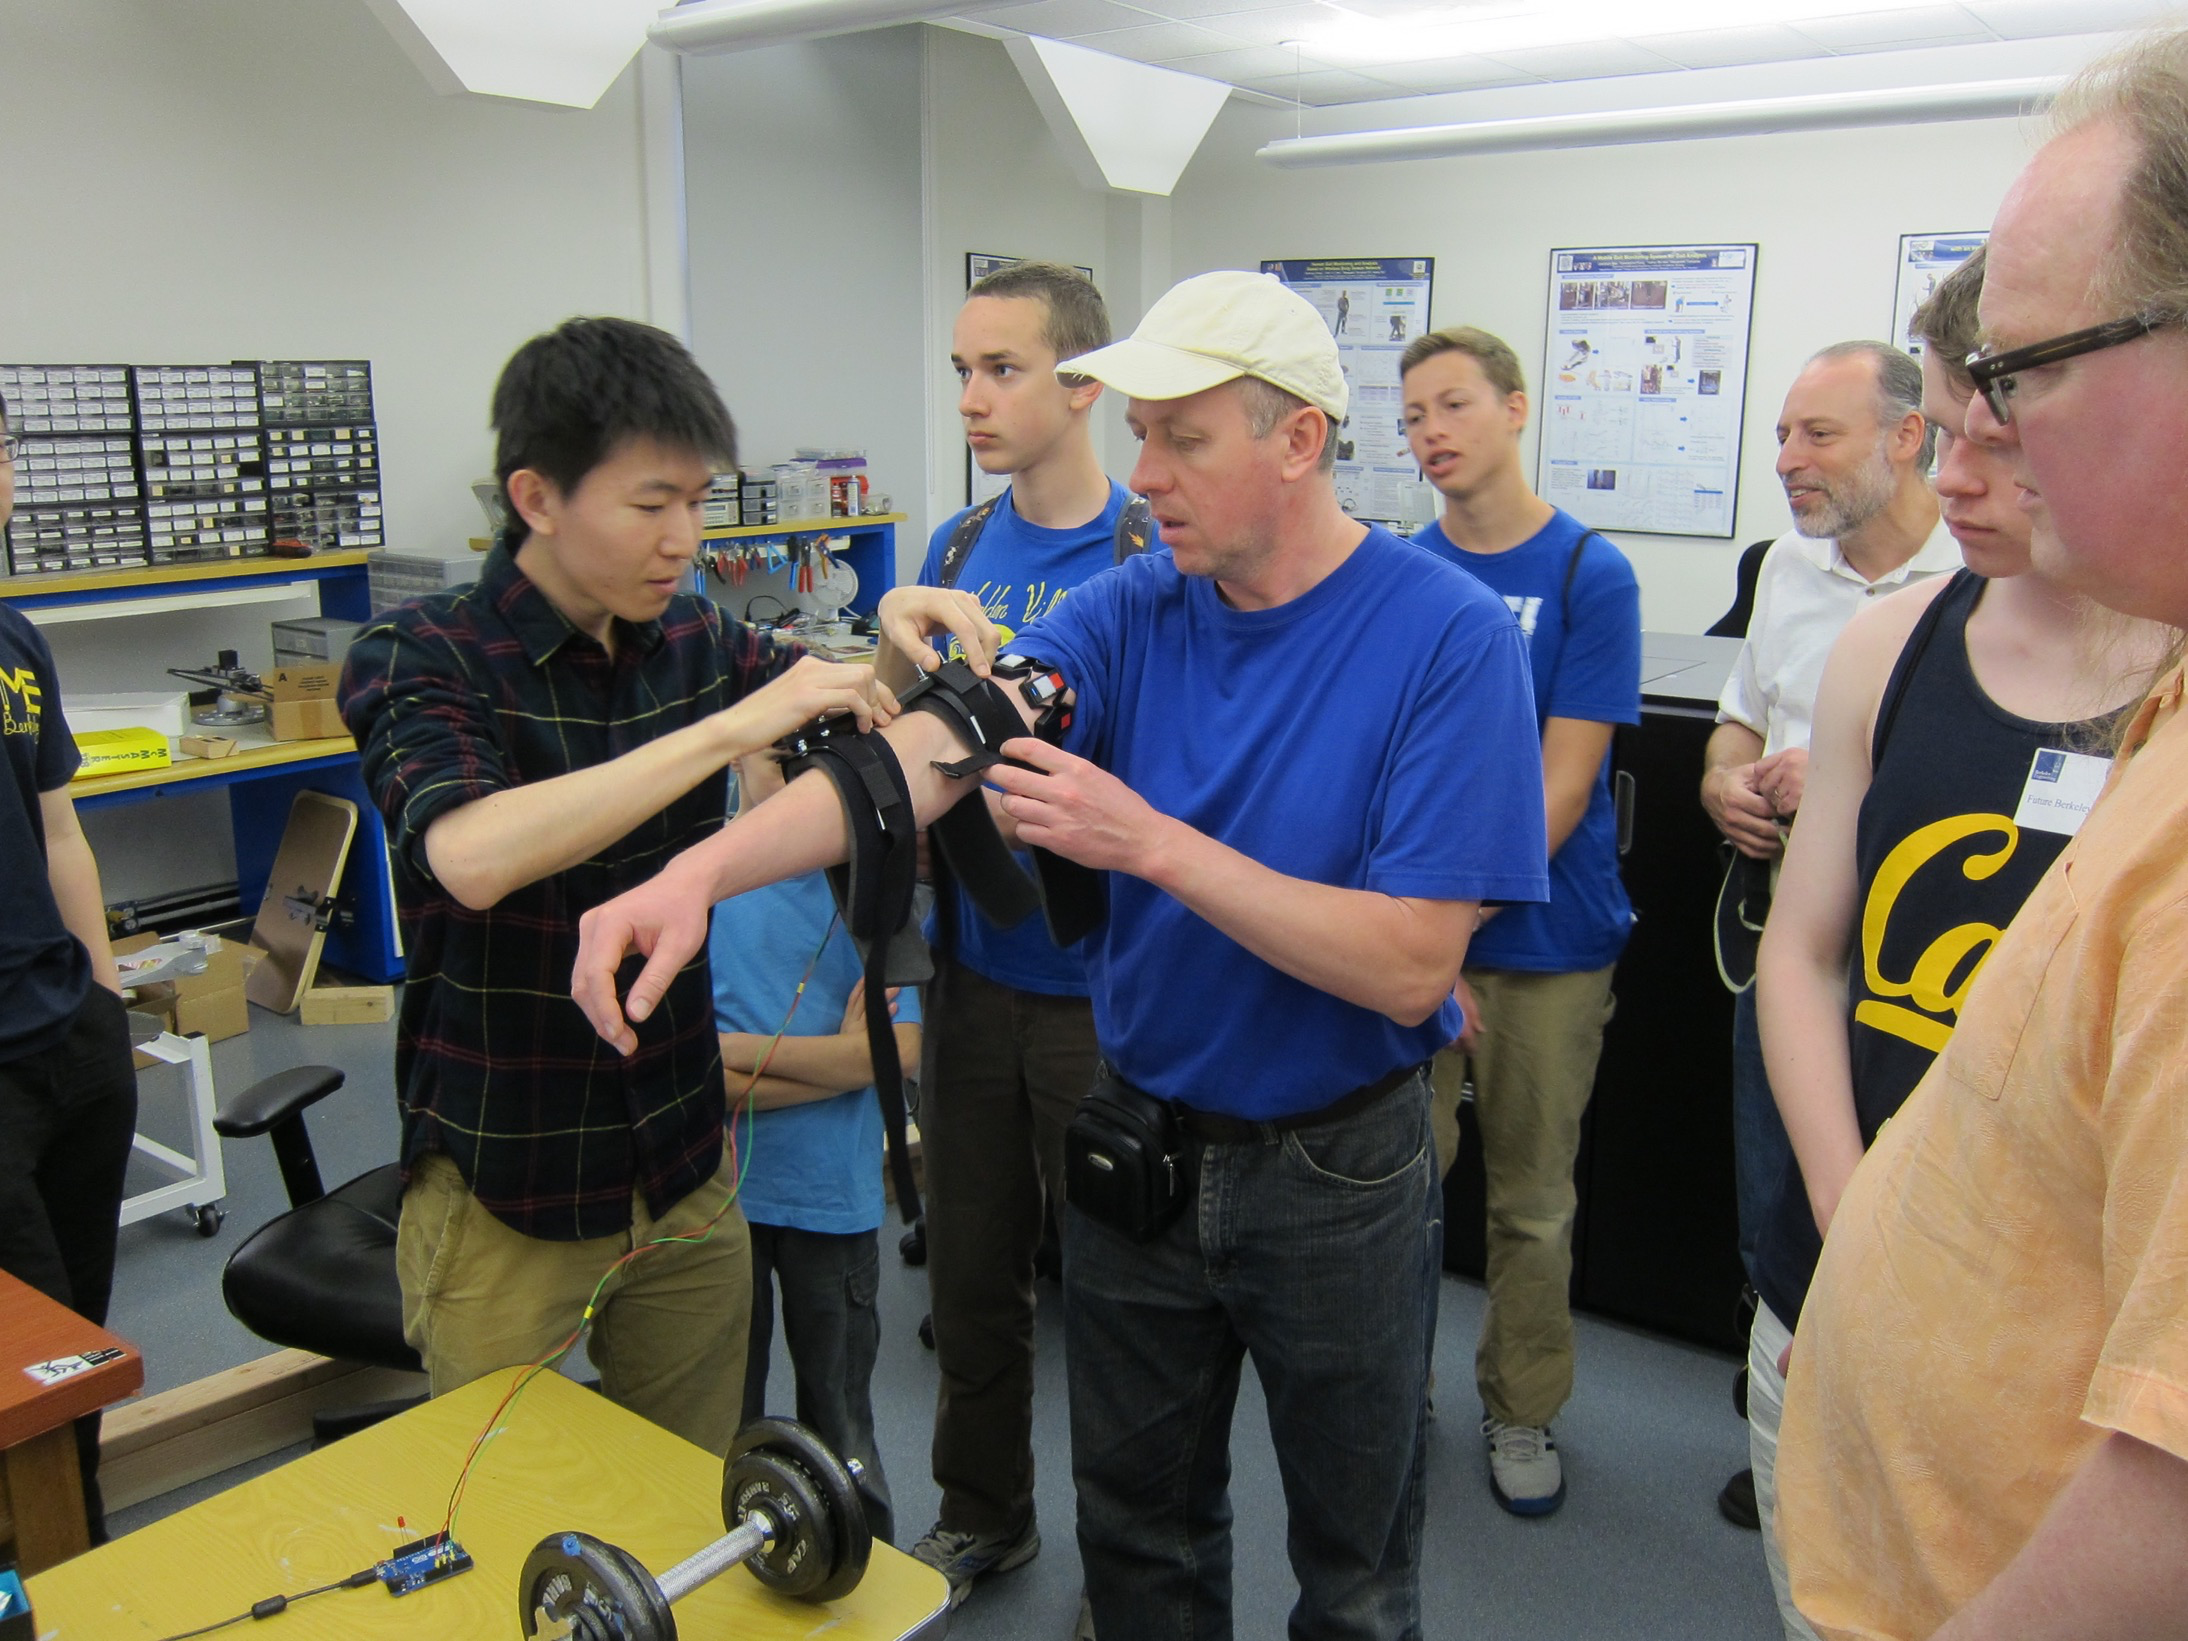
\includegraphics[width=4.5cm]{src/caldayphoto}
  \end{center}
  \vspace{-20pt}
  \caption{Cal Day 2016, a PhD student of Prof. Tomizuka demonstrating assistive technologies to visitors.\label{fig: cal day}}
  \vspace{-15pt}
\end{wrapfigure}

\paragraph*{Education Plan} ~
PI teaches robotics, design, and control courses both at the undergraduate and graduate levels emphasizing both theoretical principles and issues arising in applications of theory. His research students engage in laboratory work to acquire and develop experimental skills necessary to build, measure, and validate these new designs. 

\paragraph*{Involvement of Women and Minorities}~
The PI has a strong record in recruiting individuals from underrepresented groups, including women. While he was the Executive Associate Dean of the College of Engineering at UC Berkeley,  he was in charge of Engineering Student Services, one emphasis of which was (and still is) to broaden participation of the underrepresented groups. He has supervised twelve women to the completion of their Ph.D.s and currently supervises the Ph.D. research of nine women. 


\paragraph*{Outreach to Middle/High School Students}~
We will perform outreach to K-12 students and their parents though various official events of the University such as Cal Day (see Fig.\ref{fig: cal day} below). 
\paragraph*{Involvement of Undergraduate Students}~
Undergraduate students regularly participate in research work in the PI's lab, working closely with graduate students in projects involving hands-on experience in the fields of robotics and human mechatronics. The experimental test setups for the proposed project will provide an ideal example of interdisciplinary research, and will be made available to our undergraduate laboratory courses. The budget does not include a stipend for undergraduate researchers. We plan to request an REU supplement to attract undergraduate students from underrepresented backgrounds to the project.



\paragraph*{Broader Dissemination}~
We will disseminate the results from this research through the following mechanisms: 
(1) \textbf{Website}: Information about the group members, schedules of seminars, conferences, and workshops, copies of presentations, technical reports, code, and publications will be maintained at http://msc.berkeley.edu. The educational material, documentation, and the simulation platform developed will also be available through the website under an Open Source license. 
(2) \textbf{Journals and Conference Proceedings}: Research papers will be submitted for wide dissemination to journals and conferences in the field, such as the International Journal of Robotics Research, IEEE Transactions on Control System Technology, IEEE Intelligent Systems, IEEE Transactions of Robotics, IFAC Automatica, and ASME Journal of Dynamic Systems, Measurement, and Control.
(3) \textbf{Organized Laboratory Visits}: PI's MSC Lab regularly hosts various national and international student groups and visitors from universities and industry who will be presented with the results of the project.



\subsection{Results From Prior NSF Support}
% 5 pages or fewer of the 15 pages for entire description document.
% include results from NSF grants received in the past 5 years.
% If supported by more than one grant, choose the most relevant one.

% For each grant, include: 
%	(a) NSF award number, amount, dates of support 
%	(b) The title of this project
%	(c) Publications resulting from this research
%	(d) Summary of the results of the completed work
%	(e) A brief description of data samples available and other research products not described 	      elsewhere
%	(f) For renewed support, a description of the relationship between the completed and 			      proposed work

% Due to space limitations, it is often advisable to use citations rather
% than putting the titles of the publications in the body 
% of this section


%\paragraph*{\textit{IDR/Collaborative Research: Monitoring and Mobility Assistance with Wireless Body Sensor Network and Mechatronic Actuation}} (CMMI-1013657, September 1, 2010 - August 31, 2015, \$333,307)
%
%\textbf{Intellectual Merit}: This project studied a networked mobile assistive system (NMAS) by integrating a physical assistive device, a high-speed real-time wireless network, and a body sensor network. Major accomplishments were: 1) Prototype NMAS, 2) Control algorithms (e.g., modified LQG, model preview control, communication DOB) for a network-based rehabilitation system to deal with packet loss and varying time delay, 3) A tele-monitoring system (integration of smart shoes, IMUs, and XBee/RTWiFi/WirelessHART wireless network) for high-speed and real-time gait phase detection, and 4) Sensor fusion algorithms (e.g., time-varying complimentary filter, Direction-Cosine-Matrix estimation) using IMU sensors for accurate joint angle estimation. A preliminary clinical study conducted at the UC San Francisco demonstrated the effectiveness of NMAS in rehabilitation of patients with walking problems.
%
%\textbf{Broad Impact}: This proposed system will provide a comprehensive health care system to benefit both patients and health service providers by enabling mobile and tele-rehabilitation. Three graduate students (one of whom graduated with a Ph.D. degree), two postdoctoral researchers, and five undergraduate students have directly benefited from this project in PI Tomizuka's lab.  Four journal papers \cite{kong2012compact, bae2013tele, bae2013network, zhang2015modified} and many conference papers \cite{zhang2012modified, bae2012network, bae2012compensation, zhang2012design, zhang2013compensation, kanjanapas2013human, wei2013rt} have resulted from this project. We worked with multimedia group of the National Science Foundation to make a video of the wireless health monitoring system developed in this project \cite{nsf-video}.


\paragraph*{\textit{A Hybrid Control Systems Approach to Brain-Machine Interfaces for Exoskeleton Control}} (NSF-EFRI \#1137267, September 15, 2011 - August 31, 2015, \$2,000,000). 

\textbf{Intellectual Merit}: This interdisciplinary research addressed three major innovations (neurophysiology and brain-machine interfaces (BMI), hybrid control systems, and exoskeleton design and control) to significantly advance our understanding of fundamental principles in the neural control of movement in scenarios that involve physical interactions with the world. PI Tomizuka is mainly responsible for the third innovation (exoskeleton design and control). Major accomplishments in PI Tomizuka's lab include:
1) A passive 6-DOF upper-limb exoskeleton for macaques to test with the animals, 2) A cable-driven series elastic actuator and a torque-mode control algorithm for it, 3) An actuated version of the exoskeleton, and 4) An automatic 3D target positioner for BMI experiment use. The hybrid system approach is investigated for the BMI aspect (neural control and musculoskeletal model control).
 

\textbf{Broad Impact}: The three major innovations have been synthesized into a single new paradigm unifying the brain, biomechanics, and behavior. Two graduate students and four undergraduate students benefited from this project in PI Tomizuka's lab. The two graduate students completed their Ph.D. degrees.   Three journal papers \cite{lu2016design, lu2016interactive, haninger2016modelling} and several conference papers \cite{lu2013kinematic, haniger2014kinematic, lu2014passive, lu2014design, lu2015design, haninger2016motion, haninger2016robust} have resulted from this project. 

\paragraph*{\textit{Design of Mechanism and Control Strategies for Assistive Systems to Remedy the Decrease in Physical Strength of the Aged and the Disabled}} (CMMI \#1362172, August 1, 2014-July 31, 2017, \$307,074.00)

\textbf{Intellectual Merit}:  Integration of design and control of human assistive systems is emphasized in this research. The control problem is formulated from the viewpoint of a hybrid system. The research encompasses the segmentation of the dynamics of the human assistive system, the identification of transitions, and the development of control structures appropriate for each segment. To date, we have accomplished 1) development of a novel low-powered actuator for providing assistance; 2) Completion of a shoulder and elbow exoskeleton based on these low-power actuators; 3) Development of an algorithm for classifying the wearer's state whether the wearer has a load; and 4) Initial development of a controller for the device with the low-powered actuators by applying hybrid system theory.  Three conference papers have been published as a result of this project \cite{matthew2015introduction, matthew2015initial, matthew2015optimal}.

\textbf{Broad Impacts}: Existing work into assistive devices looks at either entirely passive assistance or fully active assistance. This new control framework uses individualized modeling to develop an active/passive actuator that can provide assistance without a large energy draw. Two Ph.D. students are working on this project and one of them graduated recently with his Ph.D. Four undergraduate students are participating.  